%%%%%%%%%%%%%%%%%%%%%%%%%%%%%%%%%%%%%%%%%%%%%%%%%%%%%
\mychapter{Questões estáticas}\label{ch:questoesClassicasMCTest}

A criação de questões estáticas é fundamental para a avaliação educacional e existem diversas abordagens e formatos disponíveis. Neste capítulo, serão abordados os dois principais tipos de questões estáticas utilizados em avaliações educacionais: as questões de múltipla escolha (QMs) e as questões dissertativas ou de texto (QTs). O objetivo é apresentar as características e particularidades de cada tipo de questão, bem como as vantagens e desvantagens de sua utilização na avaliação da aprendizagem. É importante destacar que as questões apresentadas neste capítulo não são parametrizadas, sendo as únicas variações os sorteios das questões e alternativas, no caso das QMs. No próximo capítulo, serão abordadas as questões parametrizadas.

Neste capítulo, será discutida a visibilidade do professor no menu do MCTest, permitindo que ele faça a manutenção das questões, exames e turmas que criou. Além disso, o professor também pode visualizar e utilizar questões criadas por outros professores cadastrados nas mesmas disciplinas.  É importante compreender como essa funcionalidade pode ser útil aos professores, proporcionando maior uniformidade e controle sobre as avaliações. 

\section{Tutoriais gerais sobre a navegação de questões}\label{sec:questaoNavegacao}

Na Figura \ref{fig:cap04_figQuestao}, é apresentada a lista de questões que o usuário ``fzprof'' pode visualizar ao clicar no botão ``Questões'' à esquerda do menu superior. Esse menu exibe todas as questões criadas por todos os professores cadastrados nas mesmas disciplinas de ``fzprof''.

A Figura \ref{fig:cap04_figQuestao} exibe a lista de questões, apresentando diversos atributos (colunas), como o ``Tópico'' da disciplina, o ``Tipo'' de questão (podendo ser QM ou QT), o número de alternativas (no caso do tipo QM, que neste exemplo é cinco), o ``Grupo'' da questão (para evitar que sejam sorteadas duas ou mais questões do mesmo grupo em um exame), a dificuldade variando de 1 a 5, se é paramétrica, a identificação da questão no banco de dados (``ID''), a ``Descrição curta'' (para facilitar o entendimento do que se trata a questão sem precisar abrir todo o enunciado) e, por fim, os botões de ``Ações'', que permitem atualizar ou apagar a questão. 

\begin{figure}[!ht]
  \centering
  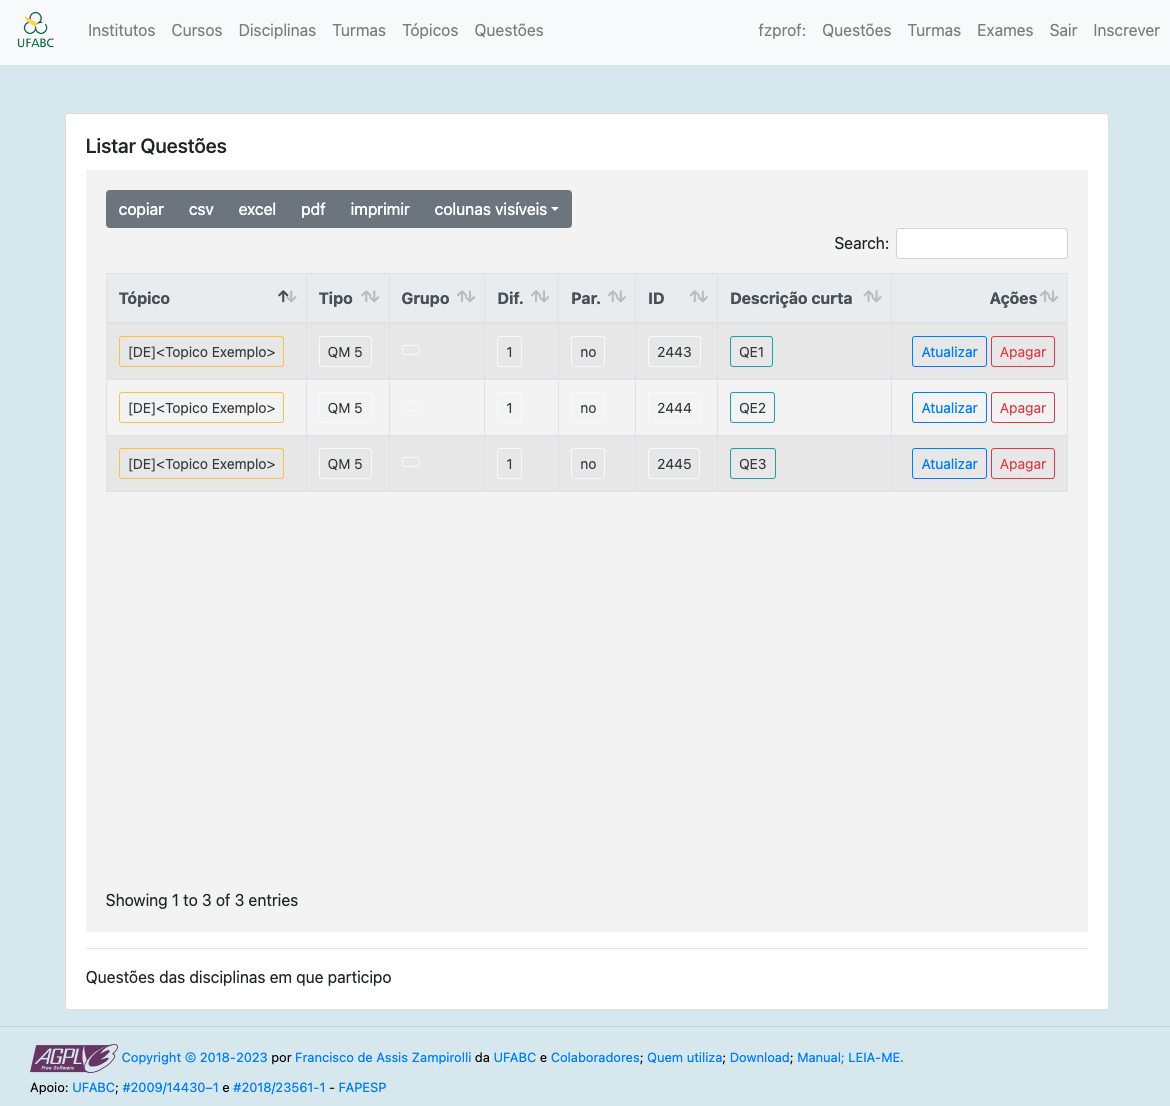
\includegraphics[width=0.9\textwidth]{cap04_figQuestao.png}
  \caption{Tela para o professor visualizar todas as questões de disciplinas que está cadastrado.}
  \label{fig:cap04_figQuestao}
\end{figure}

Caso o professor tente modificar uma questão que não é de sua autoria, será exibida a mensagem de erro apresentada na Figura \ref{fig:cap04_figQuestaoErro}.

\begin{figure}[!ht]
  \centering
  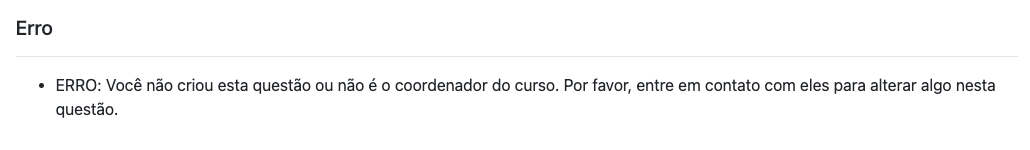
\includegraphics[width=0.9\textwidth]{cap04_figQuestaoErro.png}
  \caption{Exibição de erro ao tentar modificar questão criada por outro autor.}
  \label{fig:cap04_figQuestaoErro}
\end{figure}

\begin{mybox}{corObs}{\textbf{Observações:\\\vspace{-3mm}\hrule\vspace{1mm}}}
\begin{enumerate}
    \item Embora a Figura \ref{fig:cap04_figQuestao} exiba os botões ``Atualizar'' e ``Apagar'', é importante ressaltar que, caso o professor tente alterar ou apagar uma questão criada por outro professor, o sistema não permitirá a modificação ou exclusão da questão;
    \item É interessante manter o botão ``Atualizar'' disponível, por permitir que qualquer professor da disciplina possa visualizar como a questão foi criada. Ao clicar nas colunas ``Tipo'' até ``Descrição curta'', o professor pode conferir a questão em um modo diferente e simplificado, como mostrado na Figura \ref{fig:cap04_figQuestaoView}. É importante ressaltar que essa não é a melhor forma de visualizar os detalhes da questão, mas o professor pode acessar o PDF completo de visualização da questão clicando no botão ``Criar-PDF''.
\end{enumerate}
\end{mybox}

\begin{figure}[!ht]
  \centering
  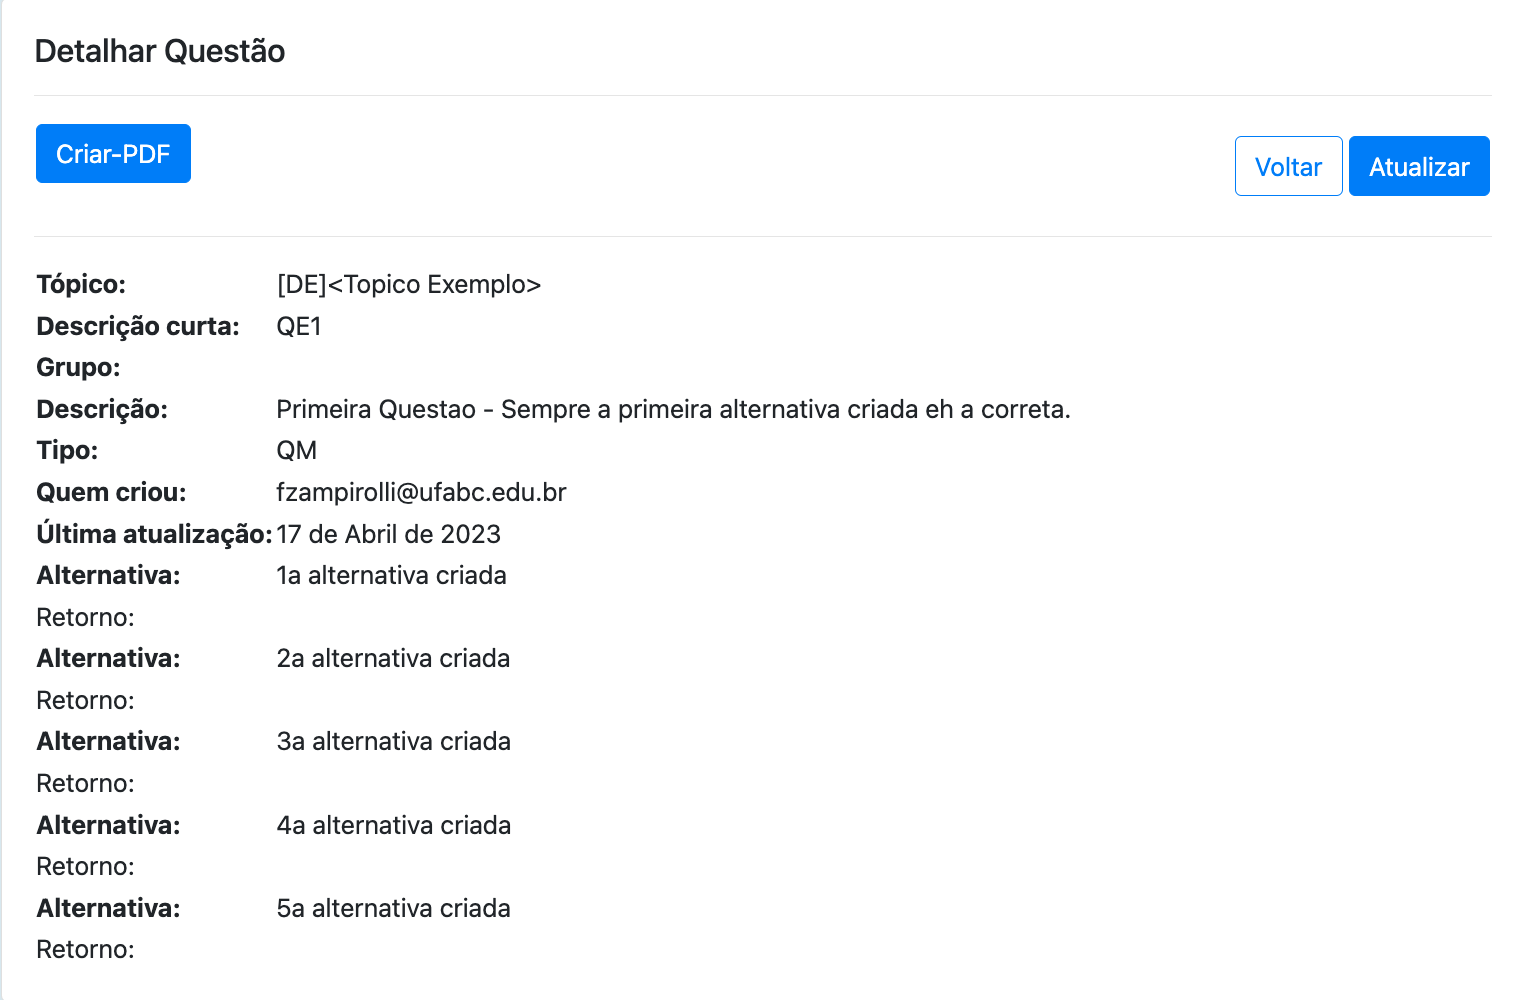
\includegraphics[width=0.9\textwidth]{cap04_figQuestaoView.png}
  \caption{Exibição da questão QE1 criada por outro autor.}
  \label{fig:cap04_figQuestaoView}
\end{figure}

Na Figura \ref{fig:cap04_figQuestaoMy}, é possível observar que o professor ``fzprof'' ainda não criou nenhuma questão. Para criar novas questões, o professor pode importar um arquivo no formato TXT, conforme exemplificado abaixo. Esse formato foi utilizado na versão 4 do MCTest, que executava no console de um computador e aceitava apenas três níveis de dificuldade: fácil (QE), médio (QM) e difícil (QH), representados em inglês por \textit{easy}, \textit{median} e \textit{hard}, respectivamente. Já a versão web atual do MCTest aceita cinco níveis de dificuldade, de 1 a 5. Ao importar uma questão de um arquivo TXT na versão web, as questões com nível de dificuldade QE terão dificuldade 1, as QM terão dificuldade 3 e as QH terão dificuldade 5.


No exemplo a seguir, o tópico é ``DE-matriz'' e é necessário existir uma disciplina com esse tópico cadastrada no MCTest. Para evitar conflitos, é recomendável incluir algum código como prefixo do tópico, como o código da disciplina. Por exemplo, ``DE-matriz'' significa que o tópico matriz pertence à disciplina ``Disciplina Exemplo'' cadastrada no MCTest. Além disso, o campo ``grupo'' da questão é importante para evitar que duas questões do mesmo grupo sejam sorteadas em um mesmo exame. Isso será exemplificado em capítulos futuros ao explicar a elaboração de exames. Finalmente, as alternativas, se existirem, devem ser precedidas de ``A:'', sendo a primeira alternativa sempre a correta. Ao visualizar uma questão, as alternativas serão sorteadas a cada vez que o PDF da questão for gerado. É possível criar várias QMs utilizando somente um arquivo TXT. Porém, se forem questões paramétricas, deve existir apenas uma questão por arquivo. 

\begin{myboxCode}{corCSV}{\textbf{Arquivo CSV, com acentos no formato \LaTeX: }}\vspace{3mm}
\hrule
\begin{verbatim}
QE::DE-matriz::grupo:: 
Crie uma matriz $3 \times 5$ de inteiros, com elementos $(i, j) = i + j$, 
com índices começando em zero, imprima a soma dos elementos da matriz.
A: 44 % alternativa correta - sempre a primeira
A: 35
A: 43
A: 55
A: 47
\end{verbatim}
\end{myboxCode}

Na Seção \ref{sec:questoesQM_QT} -- \nameref{sec:questoesQM_QT}, serão apresentados mais exemplos de como criar questões utilizando um arquivo TXT, destinadas a serem utilizadas em um exame.

\begin{figure}[!ht]
  \centering
  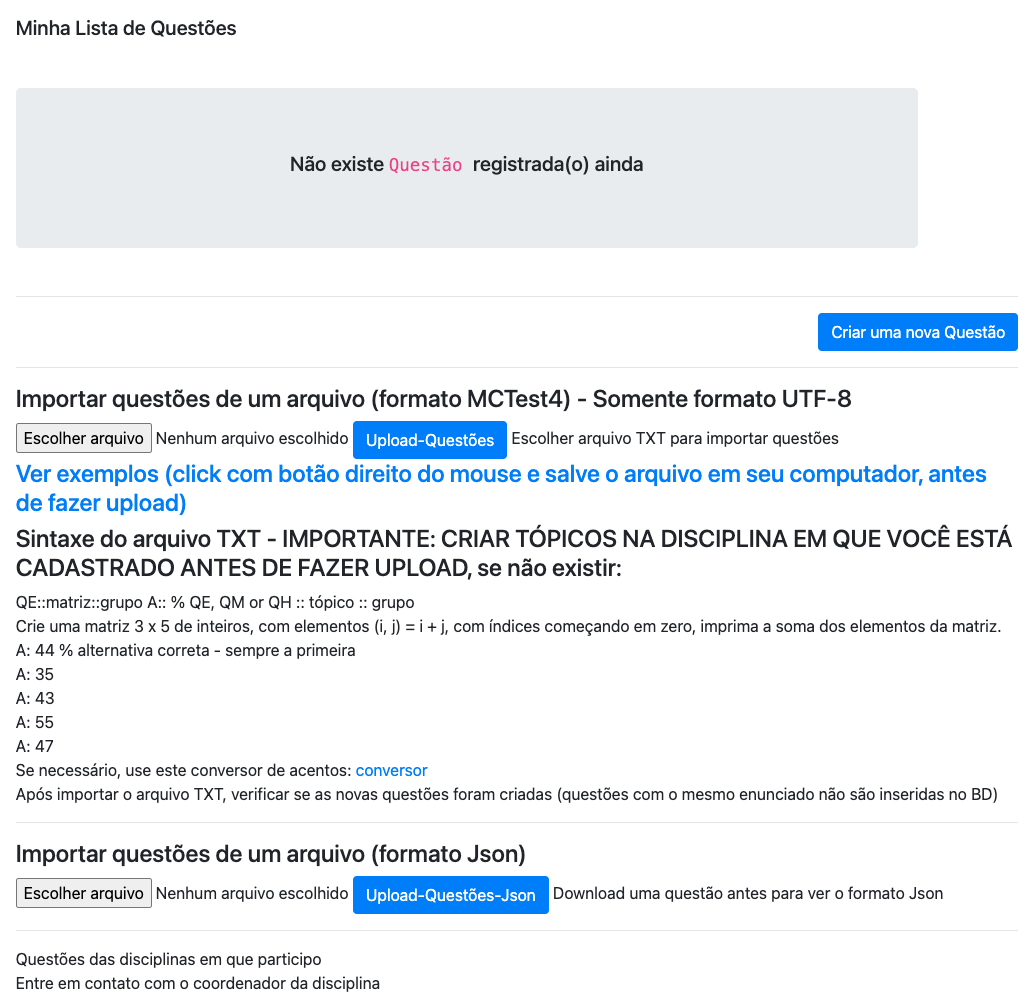
\includegraphics[width=0.9\textwidth]{cap04_figQuestaoMy.png}
  \caption{Tela para o professor visualizar suas questões e criar novas, incluindo importação de formato TXT.}
  \label{fig:cap04_figQuestaoMy}
\end{figure}

\begin{mybox}{pink}{\textbf{Melhorias:\\\vspace{-3mm}\hrule\vspace{3mm}}}
Por enquanto, o botão ``Upload-Questões-Json'' apresentado na Figura \ref{fig:cap04_figQuestaoMy} ainda não está funcionando. Essa funcionalidade será útil para um professor poder fazer \textit{backup} de suas questões e recuperá-las no futuro, caso necessário.
\end{mybox}

Em vez de criar questões por meio da importação de arquivos nos formatos TXT ou JSON, outra opção é criar as questões diretamente no MCTest. Para isso, basta clicar no botão ``Criar uma nova Questão'', apresentado na Figura \ref{fig:cap04_figQuestaoMy}. Em seguida, será aberta a tela apresentada na Figura \ref{fig:cap04_figQuestaoCria}, onde é possível criar uma nova questão. Cada questão deve pertencer a apenas um tópico, e o professor deve escolher um tópico na opção ``Escolher Tópico''. No entanto, um mesmo tópico pode ser compartilhado por mais de uma disciplina, permitindo que as questões sejam utilizadas em diferentes contextos. Em seguida, deve definir uma ``Descrição curta'' e um ``Grupo''. Também deve definir uma ``Descrição'', escolher em ``Tipo'' se é QM ou QT, escolher uma ``Dificuldade'' entre muito fácil (1) e muito difícil (5), definir a ``Taxonomia de Bloom'' e, por fim, informar se a questão é paramétrica ou não. Na Figura \ref{fig:cap04_figQuestaoCria2}, é possível ver um exemplo hipotético de preenchimento dos campos para criar uma nova questão, antes de clicar no botão ``Salvar''.

Vale destacar que ainda serão necessários incluir novos experimentos para avaliar os atributos do formulário da questão. Por exemplo, é importante analisar as características de cada questão utilizando a Teoria de Resposta ao Item (TRI) \cite{2021:Zampirolli.Junior.ea,2021:Zampirolli.Batista.ea}. Adicionalmente, a inclusão da ``Taxonomia de Bloom'' foi motivada pelos artigos de referência de \citeonline{2018:Calsavara.Serra.ea} e \citeonline{2018:Correia.Calsavara.ea}, os quais podem ser consultados na Seção \ref{sec:testeAdaptativo} -- \nameref{sec:testeAdaptativo}.

\begin{figure}[!ht]
  \centering
  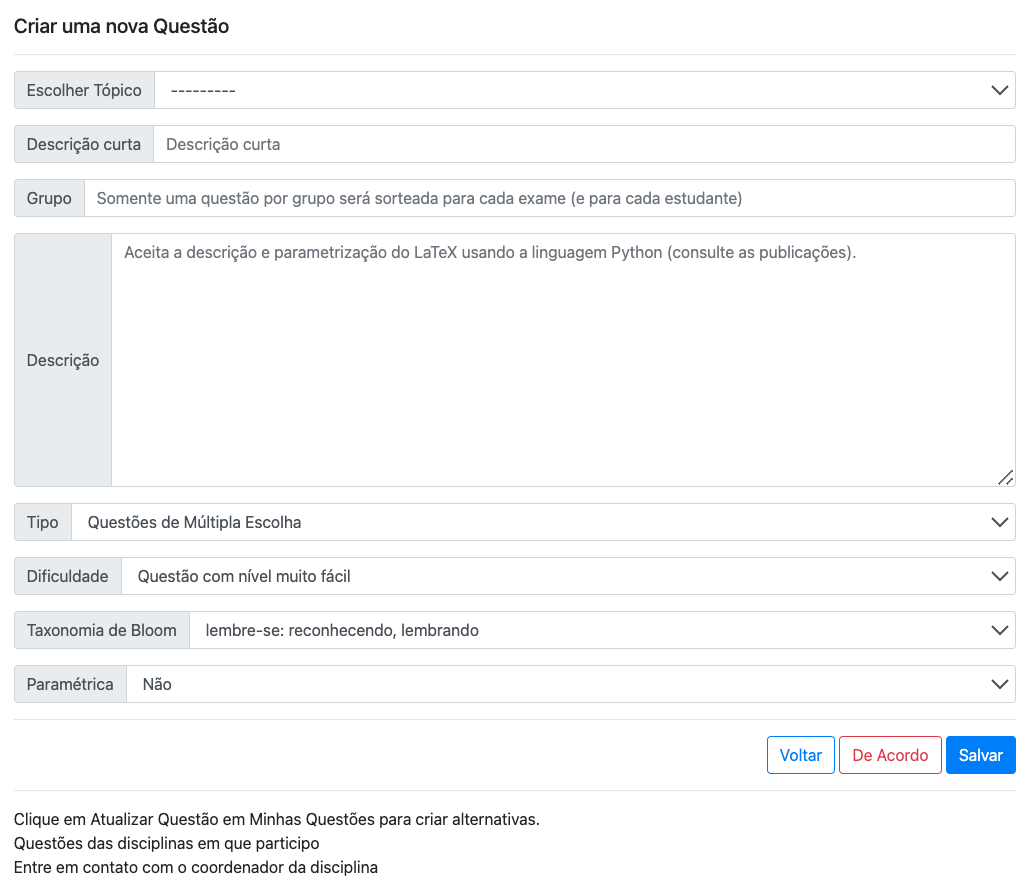
\includegraphics[width=0.9\textwidth]{cap04_figQuestaoCria.png}
  \caption{Tela para um professor criar uma nova questão.}
  \label{fig:cap04_figQuestaoCria}
\end{figure}

\begin{figure}[!ht]
  \centering
  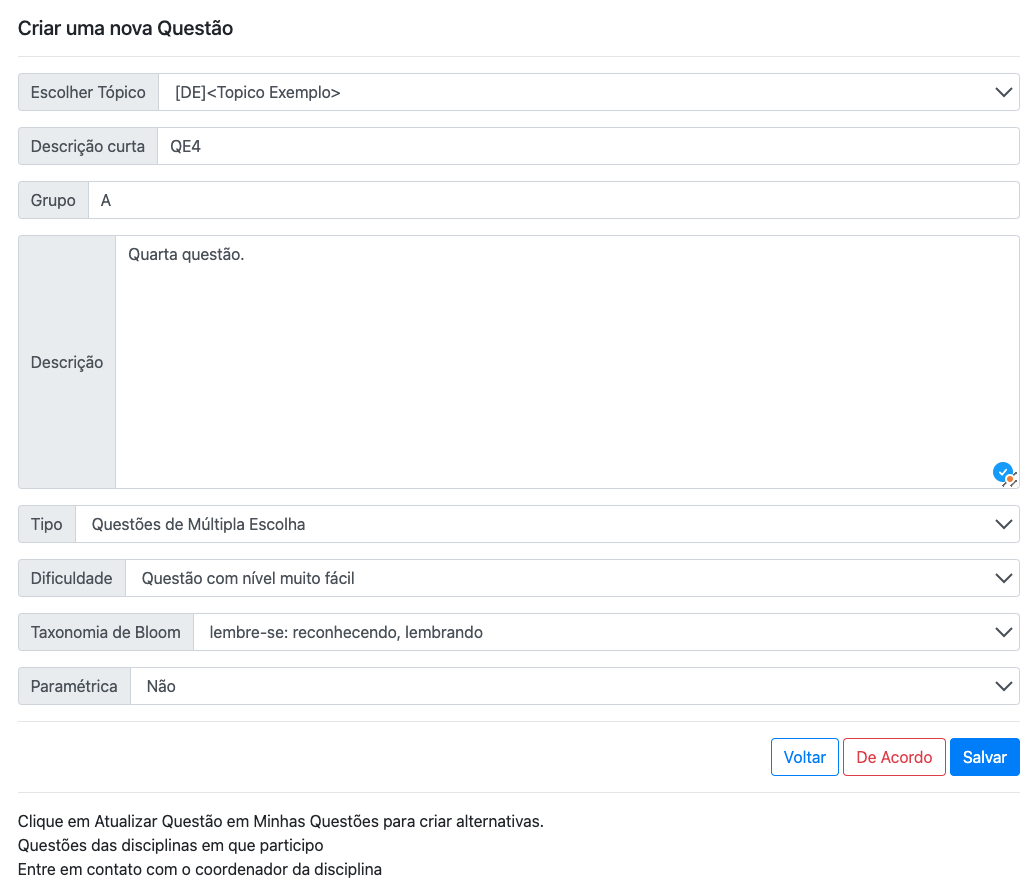
\includegraphics[width=0.9\textwidth]{cap04_figQuestaoCria2.png}
  \caption{Tela com valores preenchidos para criar uma nova questão, antes de clicar no botão ``Salvar''.}
  \label{fig:cap04_figQuestaoCria2}
\end{figure}

\section{Questão de múltipla escolha (QM)}\label{sec:questaoQM}

Nesta seção, serão abordadas as QMs, após a revisão geral das questões apresentadas na seção anterior. A QM é um tipo de questão amplamente utilizado em avaliações educacionais. Ela consiste em apresentar ao estudante uma pergunta ou enunciado, seguido de diversas opções de resposta, variando geralmente de três a cinco alternativas, das quais apenas uma é a correta. O objetivo é verificar se o estudante possui o conhecimento necessário para identificar a resposta correta dentre as opções apresentadas. O MCTest também possibilita a existência de mais de uma alternativa correta, ou a atribuição de pesos diferentes em cada alternativa, mas esses tópicos serão abordados em capítulos futuros.

As QMs são frequentemente utilizadas em testes padronizados, exames de vestibular e concursos públicos, além de serem comuns em avaliações em sala de aula. Elas são consideradas uma forma eficiente e prática de avaliar o conhecimento dos estudantes, já que permitem avaliar inúmeras pessoas em pouco tempo e com baixo custo. No entanto, uma das desvantagens desse tipo de questão é a possibilidade de plágio. O MCTest, porém, consegue minimizar esse problema com a utilização de sorteio das questões e alternativas, gerando exames individuais para cada estudante.

Após a criação da questão, realizada ao clicar no botão ``Salvar'' na Figura \ref{fig:cap04_figQuestaoCria2}, pode ser necessário atualizá-la para adicionar alternativas, caso seja uma QM. Para isso, basta acessar a opção ``Questões'' à direita de ``fzprof'', na Figura \ref{fig:cap04_figQuestao}, e, em seguida, selecionar o botão ``Atualizar'' referente à questão desejada. Será apresentada uma nova tela, conforme ilustrado nas Figuras \ref{fig:cap04_figQuestaoAtualiza} e \ref{fig:cap04_figQuestaoAtualiza2}.

Na Figura \ref{fig:cap04_figQuestaoAtualiza}, o professor pode visualizar a questão em formato PDF clicando no botão ``Criar-PDF'', mostrado na Figura \ref{fig:cap04_figQuestaoAtualizaPDF}. Ao se tratar de uma questão paramétrica que inclui códigos em Python, o professor pode testar a questão separadamente no \href{https://colab.research.google.com/}{Google Colab}, clicando no botão ``Compile-Colab''. O Colab é uma ferramenta muito útil durante a criação de questões paramétricas, já que o MCTest ainda não oferece um ambiente para compilar e depurar códigos. No entanto, esse tópico será abordado em capítulos futuros.

O botão ``Salvar-Json'' salva todas as questões criadas pelo usuário ``fzprof'' em um arquivo no formato JSON. A importação desse arquivo ainda não está disponível no MCTest, como observado anteriormente. 

Complementando a tela de criação de questões, apresentadas nas Figuras \ref{fig:cap04_figQuestaoCria} e \ref{fig:cap04_figQuestaoCria2}, a Figura \ref{fig:cap04_figQuestaoAtualiza} inclui os atributos ``Quem criou'' e a data da ``Última atualização''.  A seguir estão as políticas de edição e uso de questões no MCTest:

\begin{mybox}{corObs}{\textbf{Observações:\\\vspace{-3mm}\hrule\vspace{1mm}}}
\begin{enumerate}
    \item Somente o criador da questão ou o coordenador da disciplina podem editar uma questão;
    \item No entanto, todos os professores cadastrados na disciplina têm permissão para utilizar as questões em seus exames, se concordarem com os termos apresentados na Seção \ref{sec:deAcordo} - \nameref{sec:deAcordo}, disponível na opção ``De Acordo'' da Figura \ref{fig:cap04_figQuestaoAtualiza2}. Essa é uma política adotada na UFABC, mas outras instituições podem adotar políticas diferentes.
\end{enumerate}
\end{mybox}

Além disso, a Figura \ref{fig:cap04_figQuestaoAtualiza} apresenta campos para edição das alternativas da questão. Caso a questão seja dissertativa e possua conteúdo nesses campos, esses valores não serão utilizados ao criar exames.

É importante observar que a tela apresenta apenas uma alternativa, incluindo o ``Texto da Resposta'' e o ``Retorno'' desta alternativa'' (este último é opcional). Para criar novas alternativas, é necessário clicar no botão ``Salvar''. De maneira similar, para excluir uma ou várias alternativas já criadas, basta selecionar a caixa de seleção ``Apagar'' correspondente a cada alternativa que deseja excluir e, em seguida, clicar em ``Salvar''.

\begin{mybox}{corEdicao2}{\textbf{Destaque:\\\vspace{-3mm}\hrule\vspace{3mm}}}
As Figuras \ref{fig:cap04_figQuestaoAtualiza} e \ref{fig:cap04_figQuestaoAtualiza2} foram atualizadas para permitir que o professor efetue o armazenamento no servidor do MCTest de imagens e as inclua em uma questão. O professor pode selecionar um arquivo no formato PNG para importação, sendo necessário tomar precauções quanto ao nome do arquivo, a fim de evitar a sobreposição com outro arquivo de mesmo nome. Uma sugestão consiste em acrescentar um prefixo ao nome do arquivo, tal como \verb|fz_PDI_image01.png|. É importante observar que o nome do arquivo não deve conter caracteres especiais nem espaços em branco. Este arquivo permanecerá no servidor pelo período de 180 dias. Adicionalmente, é relevante ressaltar que a inclusão de imagens em um documento \LaTeX{} pode resultar em considerável lentidão na geração do arquivo PDF. 
\end{mybox}

\begin{mybox}{corEdicao2}{\textbf{Destaque:\\\vspace{-3mm}\hrule\vspace{3mm}}}
A Figura \ref{fig:cap04_figQuestaoAtualiza2} foi atualizada para incluir dois contadores: um para o número de correções realizadas para QM e outro para o número de questões que os estudantes acertaram. Com isso, é possível calcular a acurácia da questão (\textit{corretas/correções}). Além disso, foram adicionados os parâmetros da Teoria de Resposta ao Item (TRI): Discriminação (\(a\)), Habilidade (\(b\)) e Chute (\(c\)). Ver Seção \ref{sec:testeAdaptativo} -- \nameref{sec:testeAdaptativo} para mais detalhes do uso deste recurso.
\end{mybox}

O modelo TRI emprega uma função logística que pode ajustar até três parâmetros associados a um item (questão): a complexidade (ou habilidade), representada pelo modelo logístico de um parâmetro (\(b\), ou 1PLM, conforme mostrado na Curva Característica do Item na Figura \ref{fig:cap04_figTRI}); essa característica é combinada com a capacidade discriminativa (modelo logístico de dois parâmetros \(a\) e \(b\), ou 2PLM); e, por fim, essas características são integradas com a causalidade (acerto pelo chute) (modelo logístico de três parâmetros \(a\), \(b\) e \(c\), ou 3PLM). No estudo \cite{min2021systematic}, os pesquisadores estimam um mínimo de 200, 500 e 1.000 participantes nos modelos 1PLM, 2PLM e 3PLM, respectivamente. A Figura \ref{fig:cap04_figTRI} foi gerada através deste \href{https://colab.research.google.com/drive/1ka7_SR_QB4G7ZPVvH3p_E0bZEbOH1vhK}{Colab}.

\begin{figure}[!ht]
  \centering
  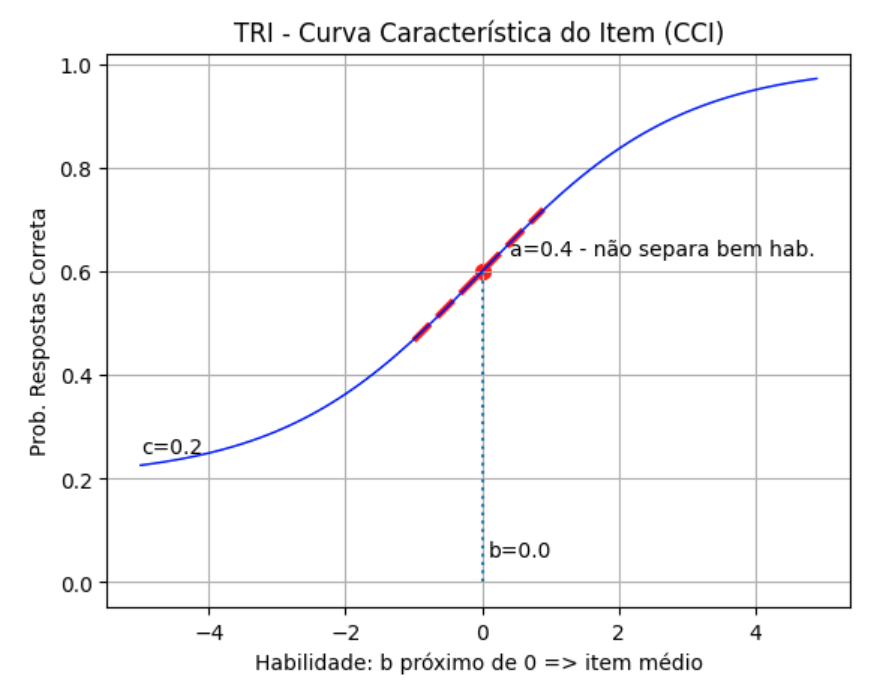
\includegraphics[width=0.9\textwidth]{cap04_figTRI.png}
  \caption{Curva Característica do Item (CCI) de 3-Modelo Logístico de Parâmetros, ou 3PLM. Adaptado de \citeonline{2021:Zampirolli.Batista.ea}.}
  \label{fig:cap04_figTRI}
\end{figure}

\begin{mybox}{corEdicao2}{\textbf{Destaque:\\\vspace{-3mm}\hrule\vspace{3mm}}}
Na Figura \ref{fig:cap04_figQuestaoAtualiza2}, há o botão ``Duplicar esta Questão'' para facilitar o processo de criar uma nova questão com base em uma já existente.
\end{mybox}

\begin{figure}[!ht]
  \centering
  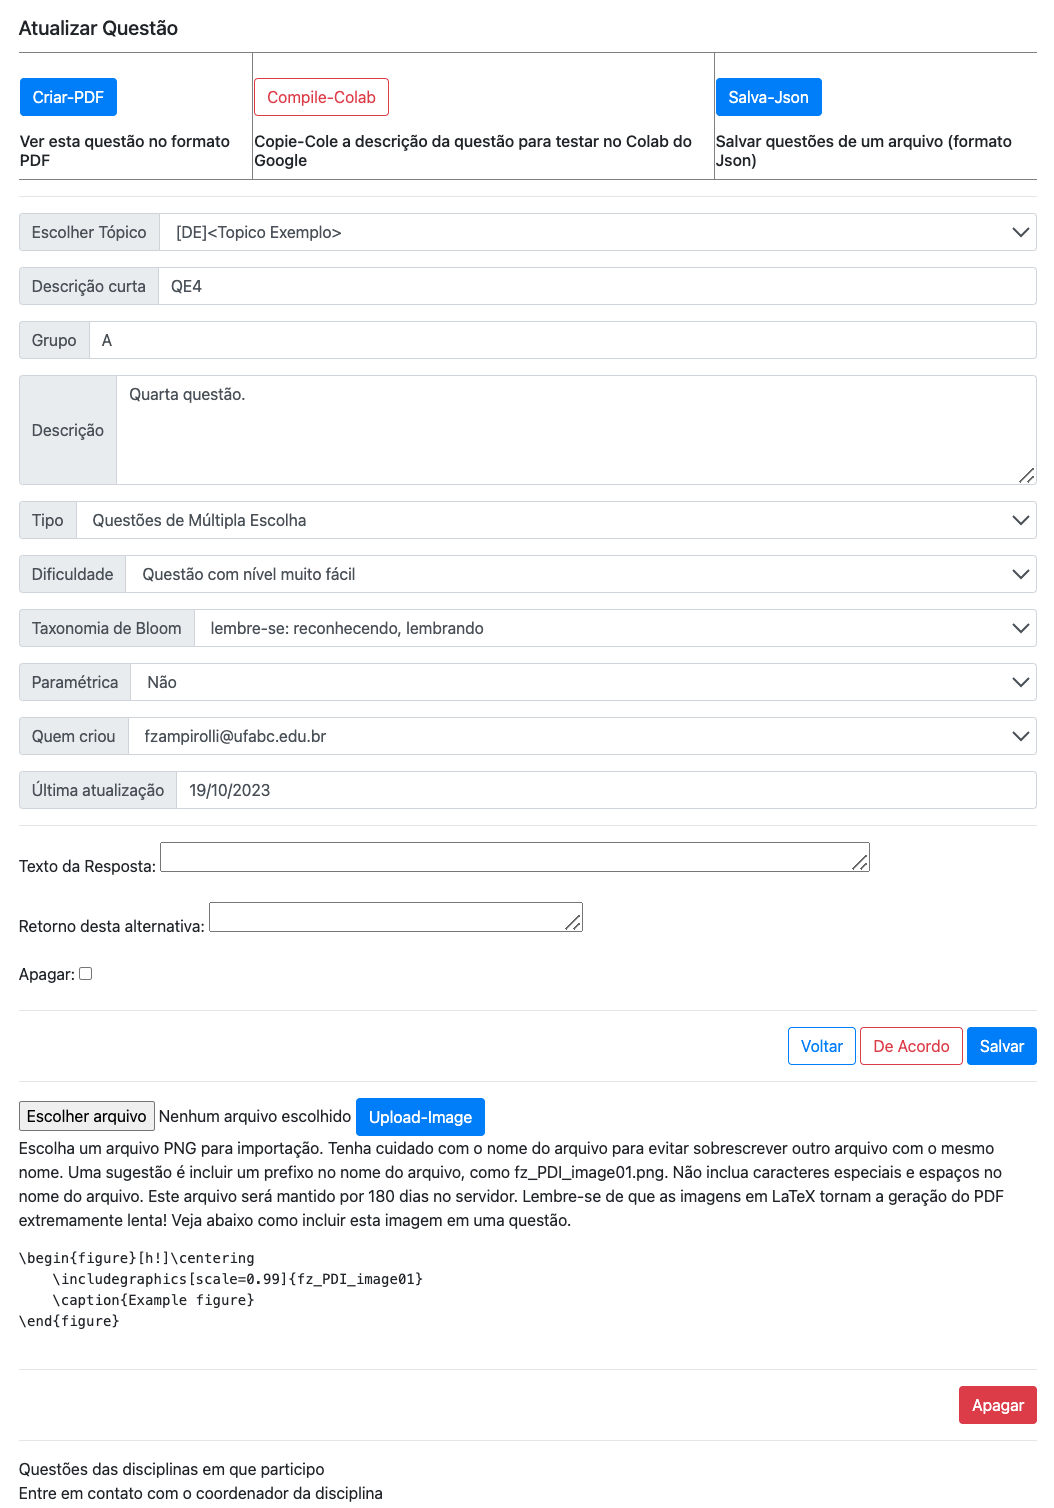
\includegraphics[width=0.9\textwidth]{cap04_figQuestaoAtualiza.png}
  \caption{(Parte 1) Tela de atualização de questão sem alternativas e \textit{feedback}, previamente criada pelo professor.}
  \label{fig:cap04_figQuestaoAtualiza}
\end{figure}

\begin{figure}[!ht]
  \centering
  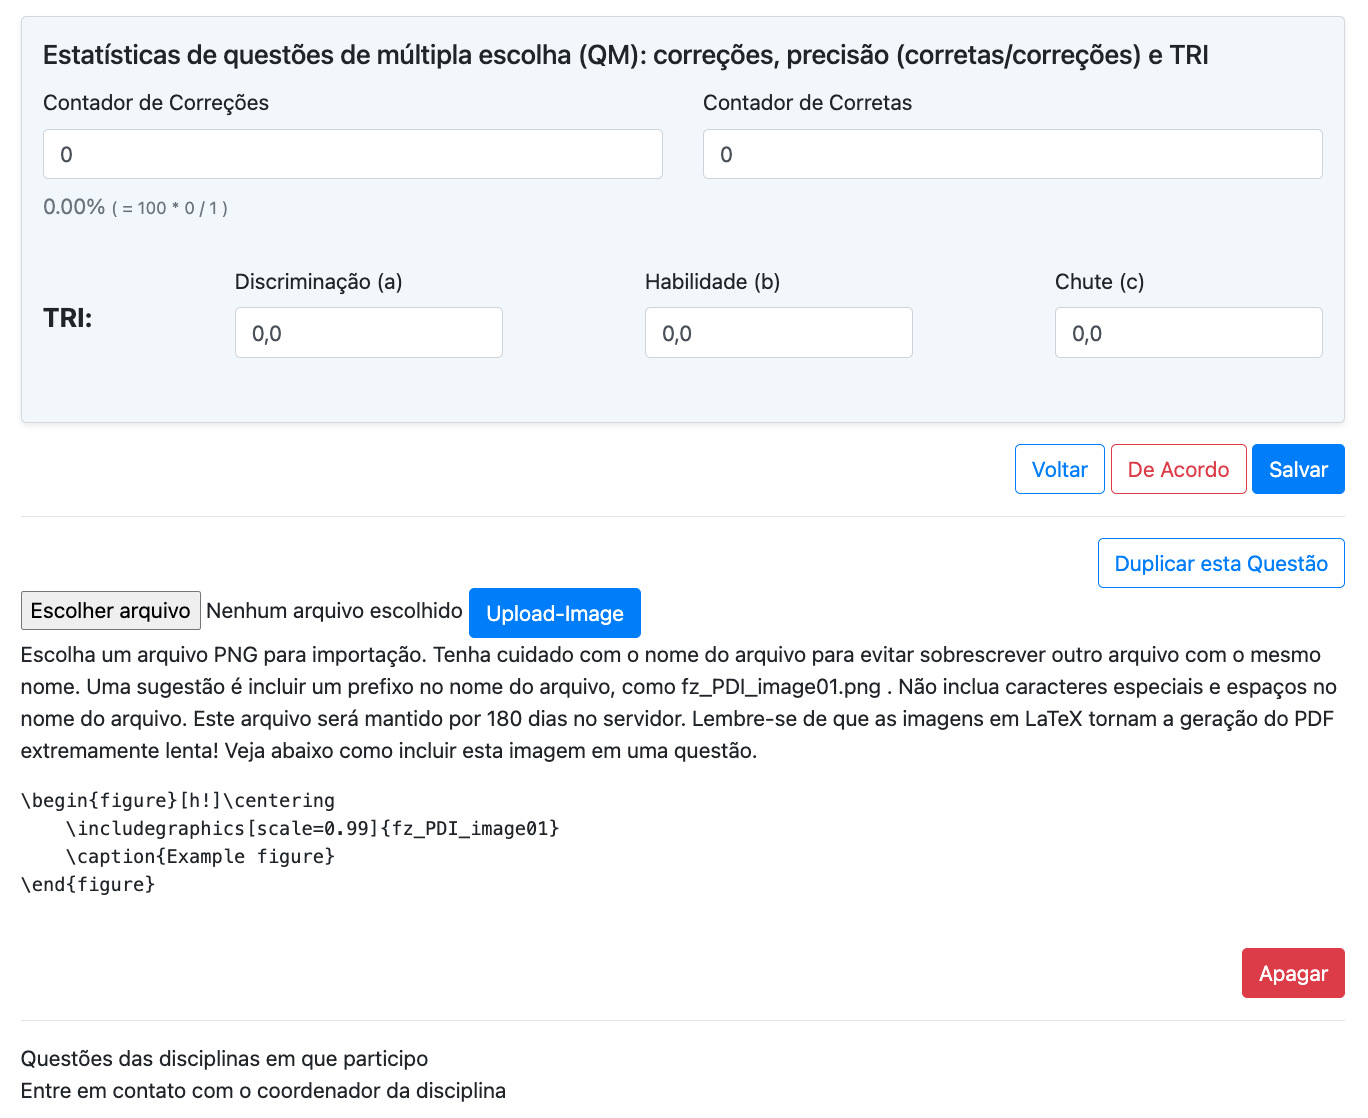
\includegraphics[width=0.9\textwidth]{cap04_figQuestaoAtualiza2.png}
  \caption{(Parte 2) Continuação da tela de atualização de questão, com estatísticas e ajuda para incluir figura.}
  \label{fig:cap04_figQuestaoAtualiza2}
\end{figure}

\begin{figure}[!ht]
  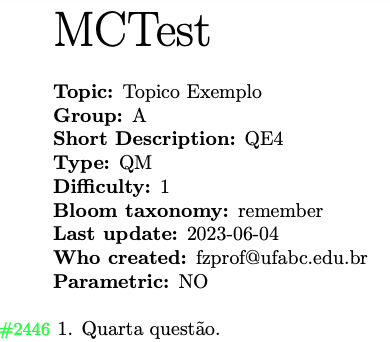
\includegraphics[width=0.35\textwidth]{cap04_figQuestaoAtualizaPDF.png}
  \caption{Recorte do PDF gerado após clicar no botão ``Criar-PDF'', na Figura \ref{fig:cap04_figQuestaoAtualiza}.}
  \label{fig:cap04_figQuestaoAtualizaPDF}
\end{figure}

A Figura \ref{fig:cap04_figQuestaoAtualizaPDF2} apresenta o PDF gerado de uma QM com cinco alternativas preenchidas, após o clique no botão ``Criar-PDF''. O número em verde representa o ID da questão no banco de dados. Os valores em vermelho correspondem às alternativas incorretas, enquanto o valor em azul representa a alternativa correta, considerando a ordem de criação das alternativas definidas na Figura \ref{fig:cap04_figQuestaoAtualiza}.


\begin{figure}[!ht]
  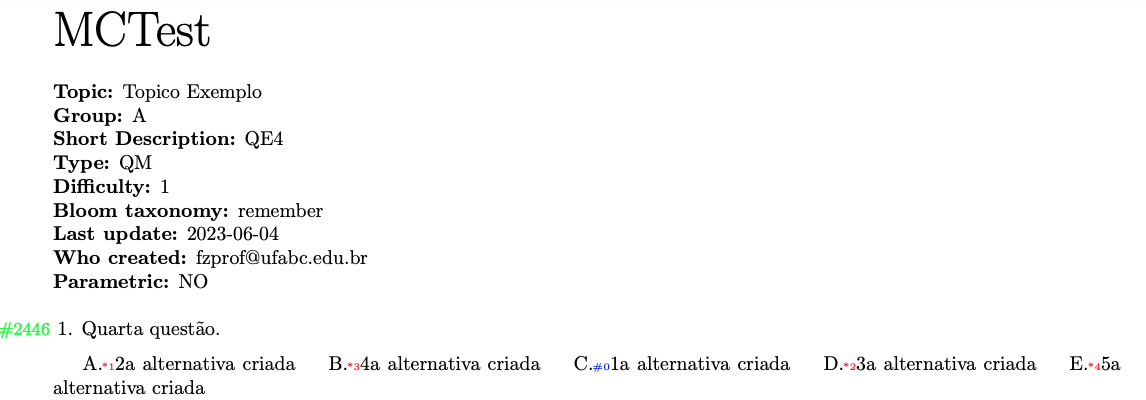
\includegraphics[width=1.0\textwidth]{cap04_figQuestaoAtualizaPDF2.png}
  \caption{Recorte do PDF gerado após clicar no botão ``Criar-PDF'', na Figura \ref{fig:cap04_figQuestaoAtualiza}, para a questão atualizada com cinco alternativas.}
  \label{fig:cap04_figQuestaoAtualizaPDF2}
\end{figure}


\section{Questão dissertativa (QT)}\label{sec:introducaoTextoQT}

Para criar uma questão dissertativa (QT -- de texto), basta selecionar a opção ``Questão Dissertativa'' no campo Tipo, conforme apresentado na Figura \ref{fig:cap04_figQuestaoCria}. É importante observar que o processo de criação para QTs é similar ao processo para QMs, apresentado na seção anterior.

A Figura \ref{fig:cap04_figQuestaoAtualizaPDF3} apresenta um exemplo de PDF gerado para uma QT. Nesse tipo de questão, o estudante deve escrever uma resposta livremente, sem a necessidade de escolher entre alternativas predefinidas. As cinco linhas que aparecem nessa questão são impressas utilizando o comando pré-definido \verb|\drawLines{5}|. É comum que as QTs sejam usadas para avaliar a compreensão do estudante sobre um determinado tema, suas habilidades de análise e argumentação, ou ainda para avaliar a sua capacidade de escrever de forma clara e organizada.

\begin{figure}[!ht]
  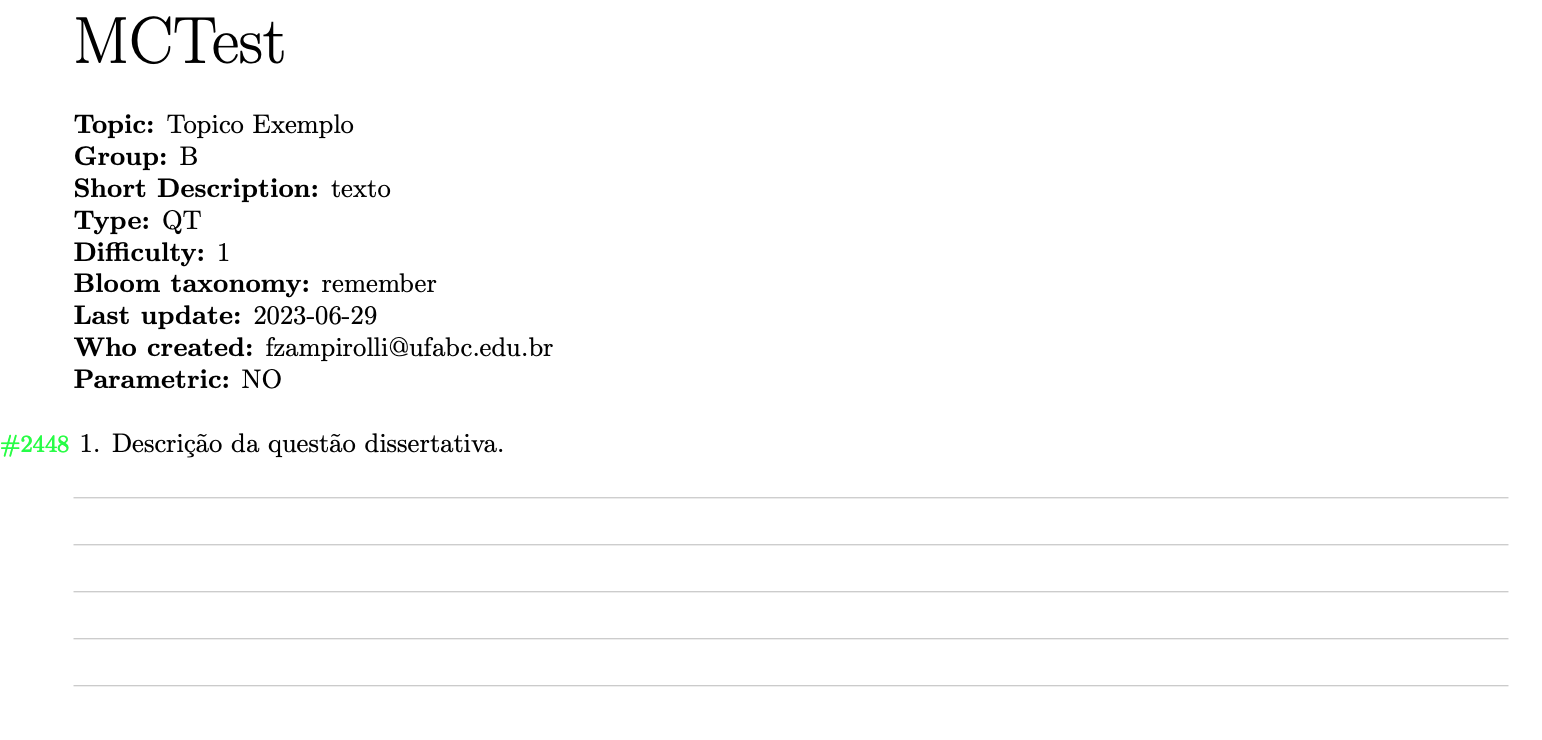
\includegraphics[width=1\textwidth]{cap04_figQuestaoAtualizaPDF3.png}
  \caption{Recorte do PDF gerado após clicar no botão ``Criar-PDF'', na Figura \ref{fig:cap04_figQuestaoAtualiza}, para uma questão dissertativa (``Type: QT'').}
  \label{fig:cap04_figQuestaoAtualizaPDF3}
\end{figure}

Na Figura \ref{fig:cap04_figQuestaoAtualizaTesteMesa}, apresenta-se a alteração do campo ``Descrição'' da Figura \ref{fig:cap04_figQuestaoAtualiza}, utilizando a sintaxe do \LaTeX, uma linguagem de marcação amplamente utilizada na produção de documentos acadêmicos. O PDF gerado desta questão é apresentado na Figura \ref{fig:cap04_figQuestaoAtualizaPDF4}

\begin{figure}[!ht]
  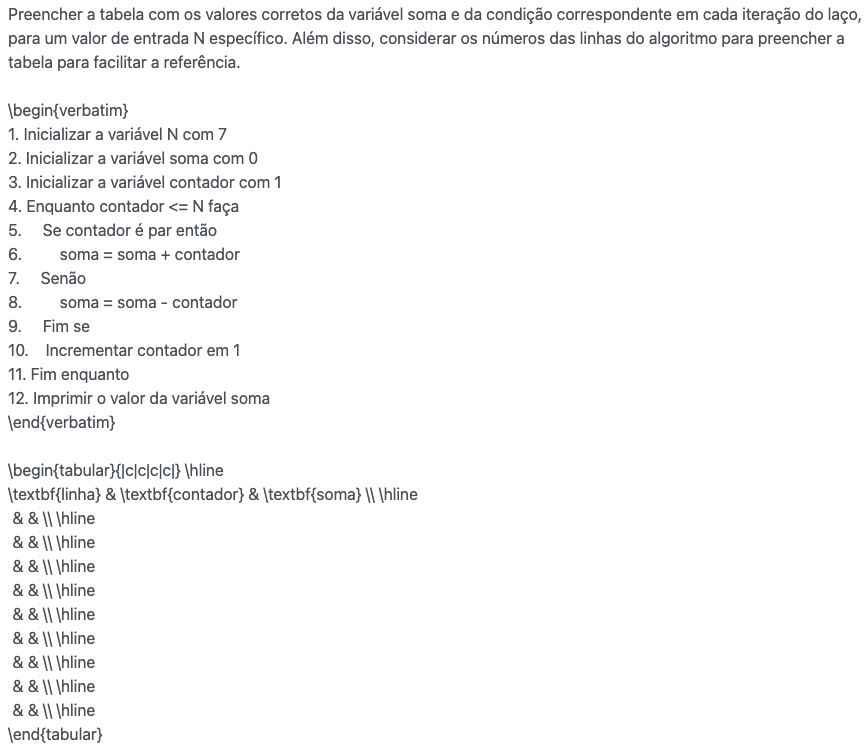
\includegraphics[width=1.0\textwidth]{cap04_figQuestaoAtualizaTesteMesa.png}
  \caption{Recorte da ``Descrição'' de uma QT de teste de mesa.}
  \label{fig:cap04_figQuestaoAtualizaTesteMesa}
\end{figure}

A questão avaliará as competências e habilidades dos estudantes em relação aos conceitos de condicional e repetição na programação. Esses conceitos são fundamentais para o desenvolvimento de algoritmos e programas computacionais, e são frequentemente abordados em disciplinas introdutórias de programação.


\begin{figure}[!ht]
  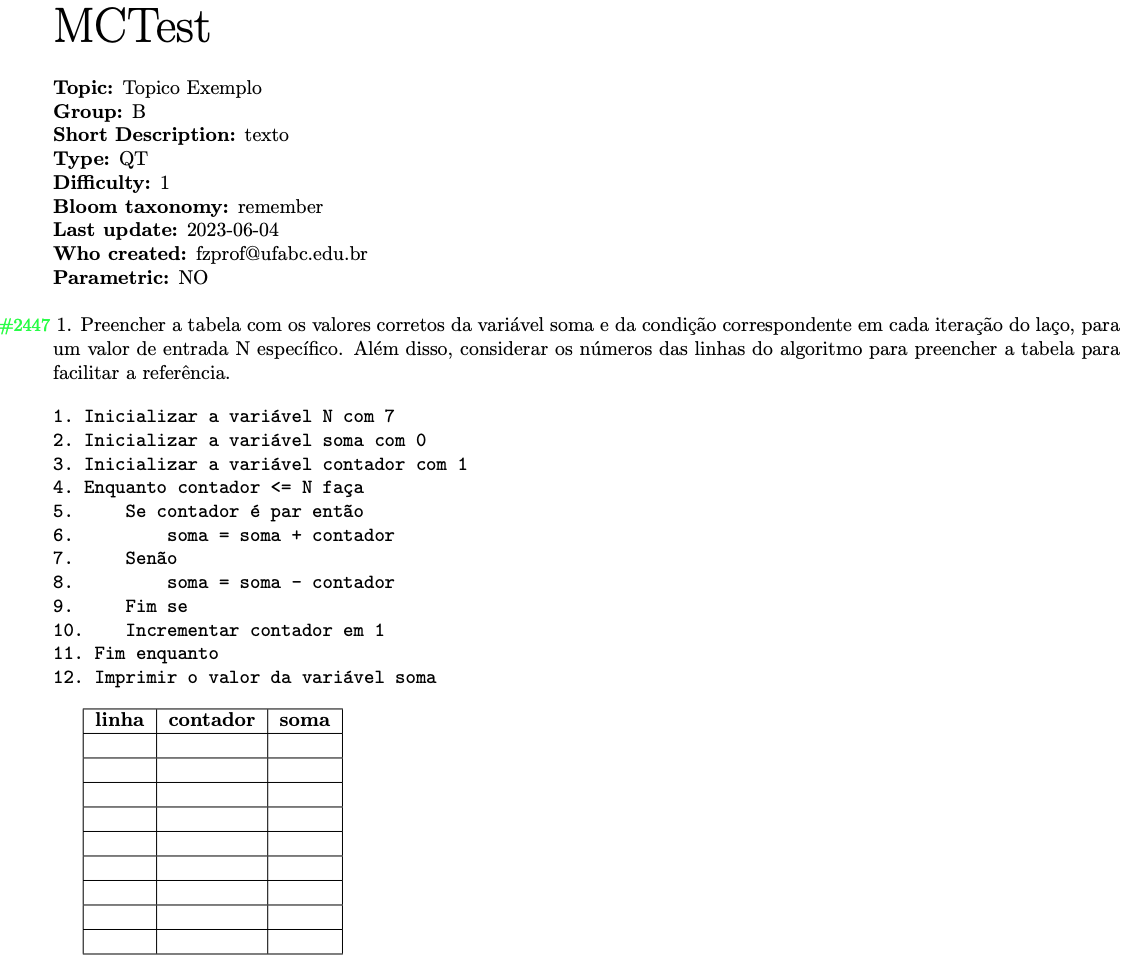
\includegraphics[width=1.0\textwidth]{cap04_figQuestaoAtualizaPDF4.png}
  \caption{Recorte do PDF gerado da QT de teste de mesa.}
  \label{fig:cap04_figQuestaoAtualizaPDF4}
\end{figure}

\section{Considerações finais}

O MCTest é uma plataforma completa que oferece diversas funcionalidades para a criação de exames. Desde QMs e QTs até questões paramétricas que envolvem códigos em Python. O MCTest oferece recursos para os professores poderem criar avaliações personalizadas para suas turmas. Além disso, a plataforma permite que as questões sejam organizadas em bancos de dados para facilitar a criação de exames.

No entanto, é importante destacar que o MCTest é apenas uma ferramenta auxiliar no processo de avaliação. A qualidade da avaliação depende não apenas das questões criadas, mas também da forma como são elaboradas e aplicadas. É fundamental que os professores sejam cuidadosos na escolha das questões e na definição do nível de dificuldade adequado para cada turma. A utilização do MCTest deve ser sempre acompanhada de uma análise crítica e cuidadosa sobre a adequação das questões e a efetividade do processo de avaliação.

Por fim, espera-se que este documento tenha sido útil para os professores interessados em utilizar o MCTest em suas disciplinas. No próximo capítulo, serão abordadas questões paramétricas que envolvem códigos em Python. 